%
% FIX THIS -- remove/change, just an example of a simple way to
%   include a lot of code (hello.c here)  
%

\chapter{Code Appendix}


\begin{figure}
    \caption{The original mutation function.}
    \begin{singlespacing} 
    \begin{small}
    \verbatiminput{mutation.rs}
    \end{small}
    \end{singlespacing}
    \label{fig:origmutation}
\end{figure}



\begin{figure}
    \caption{The function for creating a data context.}
    \begin{singlespacing} 
    \begin{small}
    \verbatiminput{newDataContext.rs}
    \end{small}
    \end{singlespacing}
    \label{fig:newdatacontext}
\end{figure}

\begin{figure}
    \caption{The function for calculating the fitness of a painting. Here, ``self'' is a painting.}
    \begin{singlespacing} 
    \begin{small}
    \verbatiminput{fitness.rs}
    \end{small}
    \end{singlespacing}
    \label{fig:fitnesscode}
\end{figure}

\begin{figure}
    \centering
    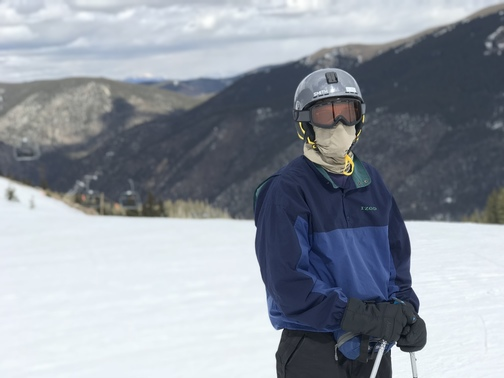
\includegraphics[width = 0.6\linewidth]{dad_pic.jpg}
    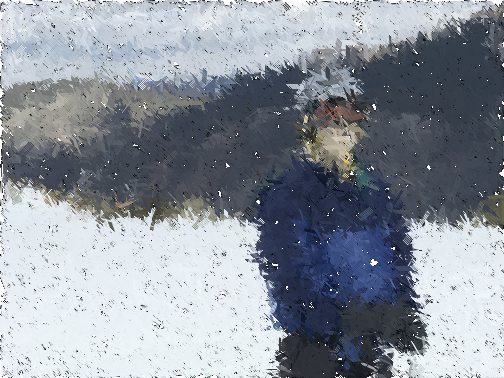
\includegraphics[width=0.6\linewidth]{dad_pic.png}
    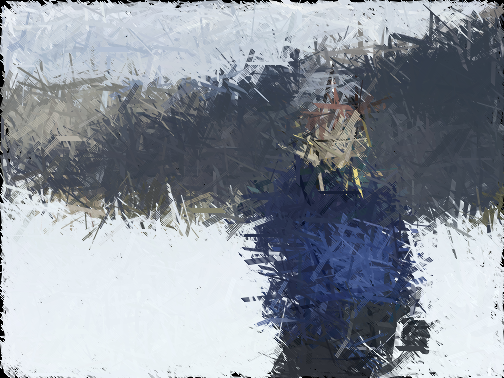
\includegraphics[width=0.6\linewidth]{dad_good_strokes.png}
    \label{fig:dadpics}
\end{figure}
\begin{figure}
    \centering
    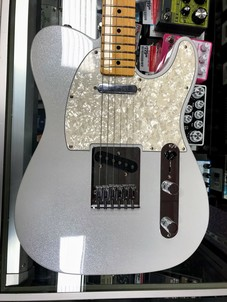
\includegraphics[width=0.4\linewidth]{guitar.jpg}
    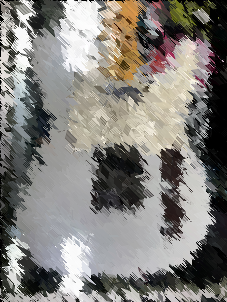
\includegraphics[width=0.4\linewidth]{big_guitar.png}
    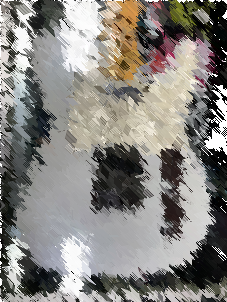
\includegraphics[width=0.4\linewidth]{guitar.png}
    \label{fig:guitarpics}
\end{figure}
\begin{figure}
    \centering
    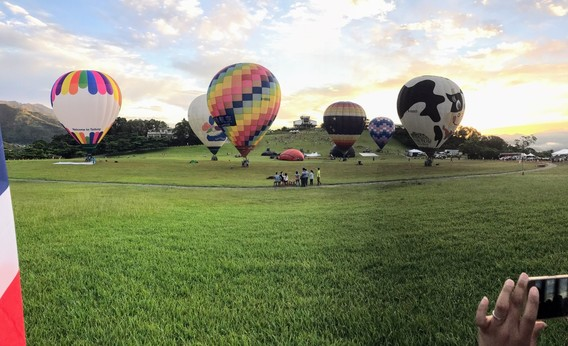
\includegraphics[width=0.8\linewidth]{hotairballoons.jpg}
    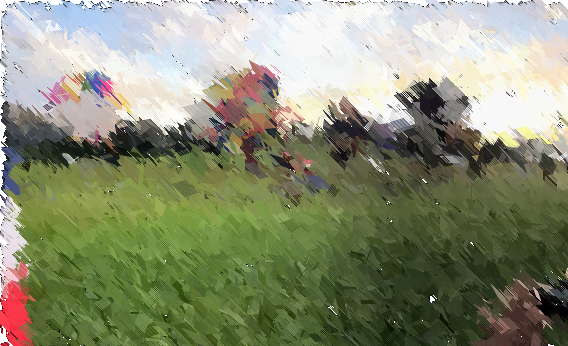
\includegraphics[width=0.8\linewidth]{hotair.png}
    \label{fig:hotairpics}
\end{figure}
\begin{figure}
    \centering
    
\includegraphics[width=0.6\linewidth]{houston.jpg}
    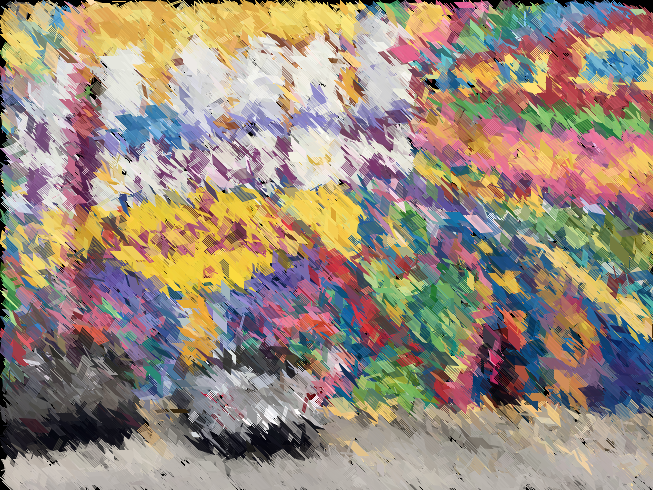
\includegraphics[width=0.6\linewidth]{houston_big.png}
    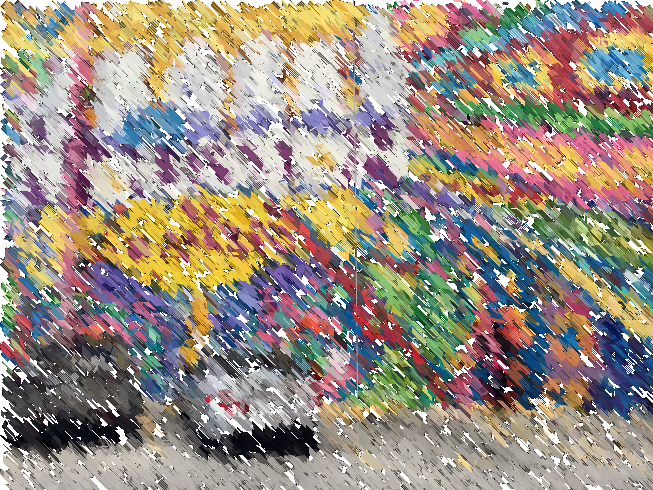
\includegraphics[width=0.6\linewidth]{houston.png}
    \label{fig:houstonpics}
\end{figure}

